%%%%%%%% EJERCICIO 8 %%%%%%
    %%%% revisar :) %%%%

    \textbf{Ejemplo 8}\\
    ¿Cuál es la tasa de interés nominal anual trimestre vencido, equivalente al 24\% nominal anual mes vencido? \\ \\
    %\newpage %USAR SOLO SI EL SOLUCIÓN QUEDA SOLO Y ES NECESARIO BAJARLO A LA SIGUIENTE PAGINA
    \textbf{Solución.}\\
    %La tabla ira centrada
    \begin{center}
      \renewcommand{\arraystretch}{1.5}% Margenes de las celdas
      %Creación de la cuadricula de 3 columnas
      \begin{longtable}[H]{|C{0.3\linewidth}|C{0.3\linewidth}|C{0.3\linewidth}|}
        %Creamos una linea horizontal
        \hline
        %Definimos el color de la primera fila
        \rowcolor[HTML]{FFB183}
        %%%%% INICIO ASIGNACIÓN PERíODO FOCAL %%%%%%%
        %%%%%%%%%% INICIO TITULO
        %Lo que se hace aquí es mezclar las 3 columnas en una sola
        \multicolumn{3}{|c|}{\cellcolor[HTML]{FFB183}\textbf{1. Asignación período focal}}                                                                   \\ \hline
        \multicolumn{3}{|c|}{$pf= \textit{No aplica}$}                                                                                                       \\ \hline
        %%%%%%%%%% FIN TITULO
    
        %%%%% INICIO DECLARACIÓN DE VARIABLES %%%%%%%
        %%%%%%%%%% INICIO TITULO
        %Lo que se hace aquí es mezclar las 3 columnas en una sola
        \multicolumn{3}{|c|}{\cellcolor[HTML]{FFB183}\textbf{2. Declaración de variables}}                                                                                             \\ \hline
        %%%%%%%%%% FIN TITULO
        %%%%%%%%%% INICIO DE MATEMÁTICAS
        %Cada & hace referencia al paso de la siguiente columna
        $j_{1}= 24\% \textit{ namv}$                                                                     & $m_{1} = 12 \textit{ pmv}$                     & $i_{2} = ?\% \textit{ ptv} $ \\
        $i_{1}= 2\% \textit{ pmv}$                                                                   &  $m_{2} = 4 \textit{ ptv} $                      &  $j_{2} = ?\% \textit{ natv} $  \\
             &       
              &  \\ \hline
    
        %%%%%%%%%% FIN DE MATEMÁTICAS
        %%%%% FIN DECLARACIÓN DE VARIABLES
    
    
        %%%%% INICIO FLUJO DE CAJA
        \rowcolor[HTML]{FFB183}
        \multicolumn{3}{|c|}{\cellcolor[HTML]{FFB183}\textbf{3. Diagrama equivalencia de tasas}}                                                             \\ \hline
        %Mezclamos 3 columnas y pondremos el dibujo
        %%%%%%%%%%%%% INSERCIÓN DE LA IMAGEN
        %Deberán descargar las imágenes respectivas del drive y pegarlas en la carpeta
        %n_capitulo/img/ejemplos/1/capitulo1ejemplo1.pdf  (el /1/ es el numero del ejemplo)
    
        \multicolumn{3}{|c|}{ 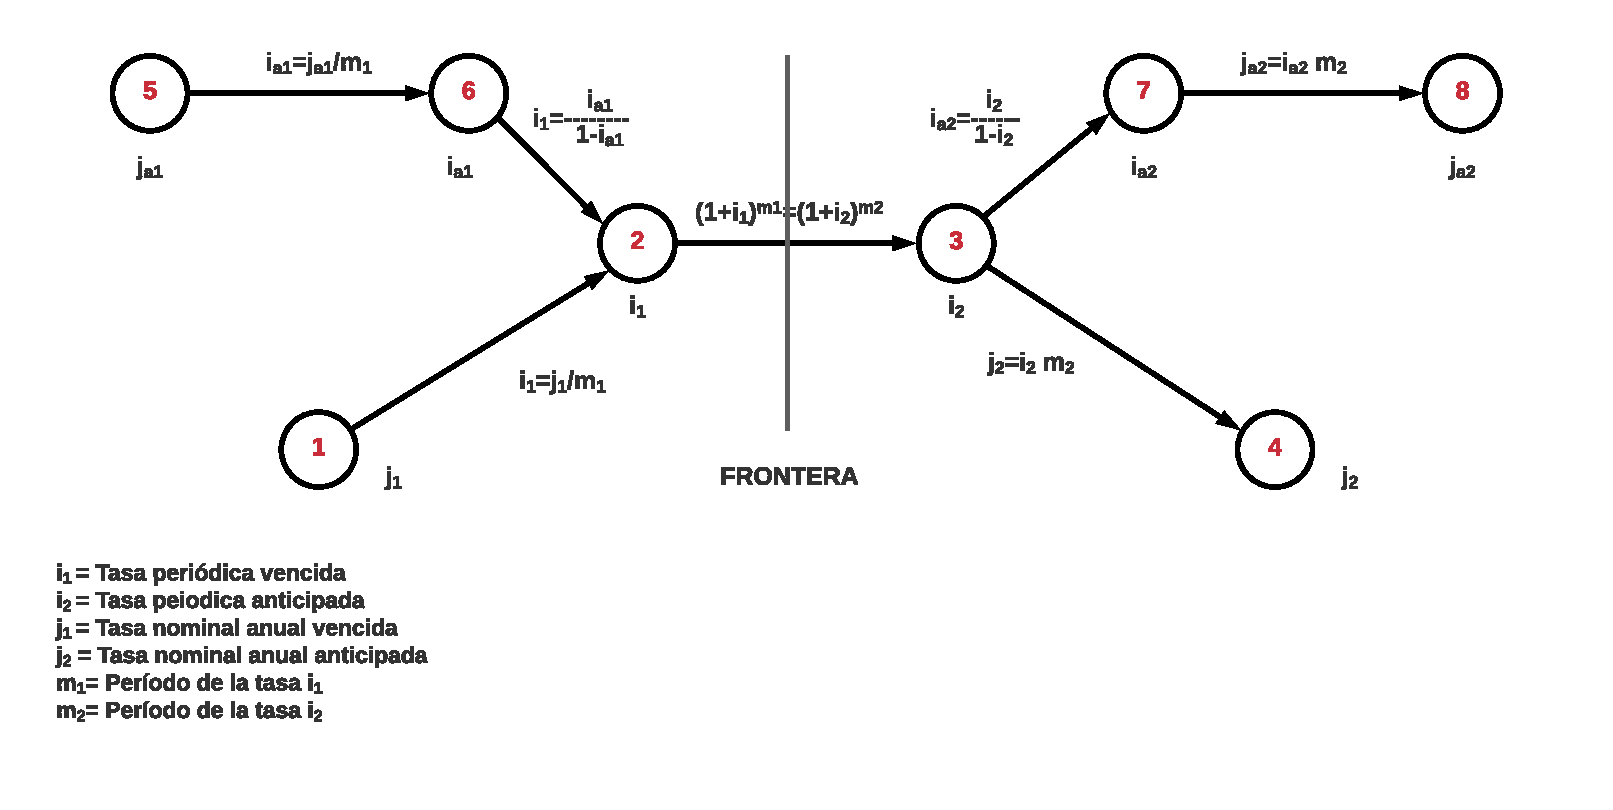
\includegraphics[trim=-5 -5 -5 -5 , scale=0.4]{2_Capitulo/img/ejemplos/6/Capitulo2Ejemplo6.pdf} } \\ \hline
        
        %%%%%%%%%%%%% FIN INSERCIÓN DE IMAGEN
        %%%%%FIN FLUJO DE CAJA
    
        %%%%% INICIO DECLARACIÓN FORMULAS
        %%%%%%%%%%% INICIO TITULO
        \rowcolor[HTML]{FFB183}
        \multicolumn{3}{|c|}{\cellcolor[HTML]{FFB183}\textbf{4. Declaración de fórmulas}}                                                                    \\ \hline
        %%%%%%%%%%% FIN TITULO
        %%%%%%%%%%% INICIO MATEMÁTICAS
    
        \multicolumn{2}{|c|}{$(1 + i_{1})^{m_{1}}= (1 + i_{2})^{m_{2}} \textit{ Equivalencia de tasas}$} & {$j_{2}=i_{2}\cdot m_{2} \textit{ Tasa nominal anual}$} \\ \hline
        %%%%%%%%%% FIN MATEMÁTICAS
        %%%%%% INICIO DESARROLLO MATEMÁTICO
        \rowcolor[HTML]{FFB183}
        %%%%%%%%%%INICIO TITULO
        \multicolumn{3}{|c|}{\cellcolor[HTML]{FFB183}\textbf{5. Desarrollo matemático}}                                                                      \\ \hline
        %%%%%%%%%% FIN TITULO
        %%%%%%%%%% INICIO MATEMÁTICAS
        \multicolumn{2}{|c|}{$(1 + 0,02)^{12}= (1 + i_{2})^{4} $}                                     & $j_{2}=(6,121\% \textit{ ptv}) (4 \textit{ ptv})$              \\
        \multicolumn{2}{|c|}{$(1,02)^{\frac{12}{4}}-1=i_{2}$ }                                          & $j_{2} = 24,48\% \textit{ natv}$                                                  \\
        \multicolumn{2}{|c|}{$i_{2}=0,061208 \textit{ ptv} \equiv$ $6,121\% \textit{ ptv}$}                                            &                                                                             \\ \hline
    
        %%%%%%%%%% FIN MATEMÁTICAS
        %%%%%% FIN DESARROLLO MATEMÁTICO
        %%%%%% INICIO RESPUESTA
        \rowcolor[HTML]{FFB183}
        %%%%%%%%%%INICIO TITULO
        \multicolumn{3}{|c|}{\cellcolor[HTML]{FFB183}\textbf{6. Respuesta}}                                                                                  \\ \hline
        %%%%%%%%%% FIN TITULO
        %%%%%%%%%% INICIO RESPUESTA MATEMÁTICA
        \multicolumn{3}{|c|}{
    
          \begin{minipage}[t][0.07\textheight][c]{0.8\columnwidth}
            \centering
            ${j_{2} = 24,48\%  natv}$
          \end{minipage}
        }                                                                                                                                                    \\ \hline
    
        %%%%%%%%%% FIN MATEMÁTICAS
        %%%%%% FIN RESPUESTA
      \end{longtable}
      %Se crean dos lineas en blanco para que no quede el siguiente texto tan pegado
      %\newline \newline %USARLO SI CREES QUE ES NECESARIO
    \end{center}
    %%%%%%%%%%%%%%%%%%%%%%%%%%FIN EJERCICIO 8 %%%%%%%%%%%%%%%%%%%%%%%%%%%
    